\documentclass[review]{elsarticle}
\usepackage{graphicx}
\graphicspath{ {pic/} }
\usepackage{lineno,hyperref}
\usepackage{amsmath}
\usepackage{natbib}
\modulolinenumbers[5]

\journal{Journal of \LaTeX\ Templates}

\bibliographystyle{elsarticle-num}
%%%%%%%%%%%%%%%%%%%%%%%
\newcommand{\dabiaolv}{reach rate }


\begin{document}

\begin{frontmatter}

\title{A data-driven approach for performance evaluation for cache group in content delivery network
    %\tnoteref{mytitlenote}
    %JPDC-A data-driven framework for performance evaluation for CDN cache groups
    }
%\tnotetext[mytitlenote]{Fully documented templates are available in the elsarticle package on %\href{http://www.ctan.org/tex-archive/macros/latex/contrib/elsarticle}{CTAN}.}

%% Group authors per affiliation:
\author{None
    %\fnref{myfootnote}
    }
\address{Radarweg 29, Amsterdam}
%\fntext[myfootnote]{Since 1880.}

%% or include affiliations in footnotes:
\author[mymainaddress,mysecondaryaddress]{Elsevier Inc}
\ead[url]{www.elsevier.com}

\author[mysecondaryaddress]{Global Customer Service\corref{mycorrespondingauthor}}
\cortext[mycorrespondingauthor]{Corresponding author}
\ead{support@elsevier.com}

\address[mymainaddress]{1600 John F Kennedy Boulevard, Philadelphia}
\address[mysecondaryaddress]{360 Park Avenue South, New York}

\begin{abstract}
CDN Service providers are increasingly using data-driven mechanisms to build their performance model of their service-providing systems. To build a model to accurately describe the performance of the existing infrastructure is very crucial to make resource management decisions. Conventional approaches that use hand-tuned parameters has its drawback. Recently, data-driven paradigm have been shown to greatly outperform traditional methods in many applications, in both accuracy and their quick reactions to the changing environment. We design a framework that using these techniques to build a performance model. Our approach shows an average 6.98\% improvement in terms of weighted mean absolute percent error (WMAPE) compared to the baseline models.
\end{abstract}
\begin{keyword}
\textit{edge computing, deep learning, content delivery networks, sequence learning, predictive analysis, high dimensional data}
%\texttt{elsarticle.cls}\sep \LaTeX\sep Elsevier \sep template
%\MSC[2010] 00-01\sep  99-00
\end{keyword}
\end{frontmatter}
\linenumbers
\section{Introduction}
% the detail of absract
The CDN Service providers are increasingly using data-driven mechanisms to build their performance model of their service-providing systems. To build a model to accurately provice an understanding of the performance of the existing infrastructure such as the health of cache groups and network status, is very crucial to make resource management decisions including content placement, network traffic scheduling, load banlance of the CDN network.

The state-of-art methods are typically using simple huristics.

%Resouoce management involves modeling the status of all available physical resources,based on which to maximize a resource utilization in terms of cost, energy performance\cite{Mistral}, overall profit,etc, and finally request allocation, and workload allocation.

There is a trend \cite{Jiang2017Pytheas:Exploration-Exploitation} \cite{Mao2017NeuralPensieve} that using data-driven methods to model complex networked systems. Traditional approach typically simple huristics. These methods have several drawbacks  \cite{Mao2017NeuralPensieve}. They cannot quickly respond to the change of the environment. the mothods, changing environment. They cannot accurately reflect and oversimplified the complex systems due to the lack of knowledge of real-word environment. VM Scheduling. Internet Telphony. CDN selection. Models that accurately describe the complex networked system

In this paper, we provide a framwork for performance evaluation for cahce groups of edge-computing. 

the relationship between CDN and edge computing (the earliest form of edge computing). A content delivery network (CDN) is a globally distributed network system deployed across the Internet. Composed with geographically distributed cache servers, CDNs deliver cached content  to  customers  worldwide  based  on their geographic locations. Extensively  using  cache  servers,  content  delivery over  CDN  has  low  latency  and  high  reliability,  and  supports better quality of experience.

In recent year, with the development of AI and data analytics system, it’s a trend using data data-driven techniques to optimize networked systems. Driven by the opportunity to collect and analyze data (e.g., application quality measurement from end users), many recent proposals have demonstrated the promise of using data-driven optimization of networked systems. Drawing parralel from the success of deep-learning. Instead of using empirical non-linear model to descirbe the complex interaction of different features, we use machine learning models and treat networked systems as a black-box.

Our prediction consists of stages: (1) feature selection (2) feature embedding (3) fully connected network/ svm/ other black-box machine learning algorithm to output the predictions. 
%\deep-learning
lstm,lstm auto encoder and decoder

Our main contributions are listed below:
\begin{itemize}
  \item data-driven approach
  \item performance modeling as sequence modeling problem
  \item anomaly detection(Collective Anomalies a) and prediction
\end{itemize}

first build a prediction model, and then use the prediction model to do the anomaly detection.

The remain organization of this paper is as follows. In Section II, we 
first  describe  the performance evaluation problem
and  then  introduce  our  LSTM  based  structure.  In  Section
III, we introduce anomaly detection algorithms based on the
auto-encoder and decoder. In  Section  IV,  we  demonstrate
performance  improvements  over baseline models. 
Finally, we provide concluding remarks in Section V.
%\cite
\section{Background}
\subsection{CDN architecture}
\subsection{cache group}
\begin{figure}[h]
    \centering
    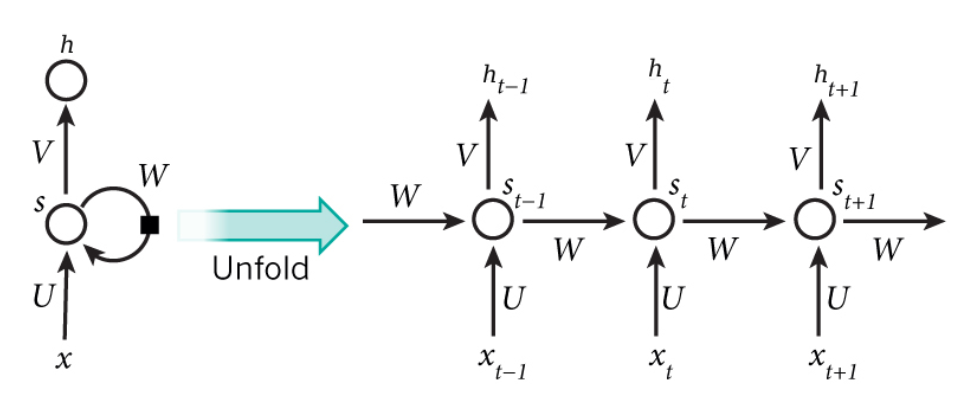
\includegraphics[width=0.5\textwidth]{RNN.png}
    \caption{}
    \label{fig:RNN}
\end{figure}
\subsection{Limitations of prior approaches}
\subsubsection{inaccuracy}
  The underlying systems are complex and often impossible to model accurately. For instance, in cluster scheduling, the running time of a task varies with data locality.
\subsubsection{unable to adapt to the change of the environment}


\section{Problem formulation and Model}
\subsection{\dabiaolv prediction}
\dabiaolv is a indirect measurement of customer QoS
\subsection{Model: performance evaluation problem formulation}
we argue that performance modeling as a sequence problem. 
Since we are able to collect the machine performance metrics and network metrics at a certain time interval, we can use a sequence models to describe relationship between machine performances and \dabiaolv
\section{}
There are four catogories of sequence learning problem, which are many to one, many to one and many one. 
Our goal is to predict the future \dabiaolv based on the metrics collected by the monitors. In general, we can use the following formulation to describe the prediction process.
\begin{equation}
	\mathbf y_t = f(x_t,x_t-1,...,x_t-p)
\end{equation}

which is many to one    
The training phase is to learn a best function that minimizes
the prediction error as follows:

\begin{equation}
	\mathbf h_t = \tanh(\mathbf W * \mathbf h_{t-1} + \mathbf I * \x_t)
\end{equation}

Many models can be used to approximate f in sequence modeling. Conventional approaches includes ARMA and its variants like ARIMA
and FARIMA. In ARMA models, the relationship between the
predictor and the target variable is simply described using a
linear model as follows:
\begin{equation}
	\mathbf h_t = \tanh(\mathbf W * \mathbf h_{t-1} + \mathbf I * \x_t)
\end{equation}
where α i and β j are coefficients that can be easily learnt by Least Square Regression.

Linear models are easy to implement and have good in-
terpretation and thus are widely used in many real work
time series analysis problems. However, linear models are
shown not sufficient to describe some nonlinear behaviors of
the network traffic. We use deep learning as alternaives.

Deep Learning (DL) is a rapidly growing discipline that, during the last few years, has revolutionalised machine learning and artificial intelligence research due to the availability of labeled data , programming framework like tensorflow, and accelerators like GPU.

 The essence of DL is to compute hierarchical features or representations of obser-vational data, where the higher-level features or factors are defi ned from primary lower-level measurements. Based on the features extracted from the data in the training set, the calculations within the model are adjusted so that known inputs produce desired outputs

deep learning (Relatively recently,sequence modeling based on LSTM technique gained popularity due to its features including automatic feature extraction abilities.\cite{Zhu2017DeepUber})

\subsection{deep learning in sequence learning}
Sequence prediction often involves forecasting the next value in a real valued sequence or outputting a class label for an input sequence.
\
\subsubsection{RNN}
%The promise of recurrent neural networks is that the temporal dependence and contextual
%information in the input data can be learned.
\cite{Bengio1994LearningDifficult}
\cite{ChoLearningTranslation}

what is RNN and RNN applied in sequence forecast.

\begin{figure}[h]
    \centering
    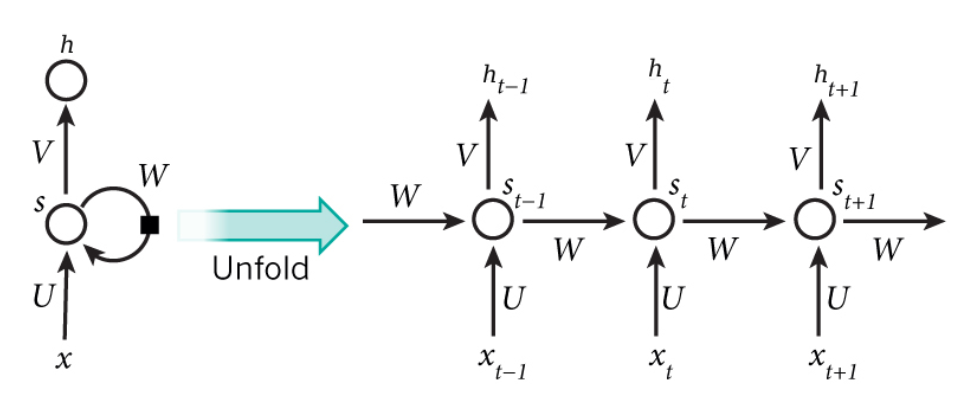
\includegraphics[width=0.5\textwidth]{RNN.png}
    \caption{RNN Architecture}
    \label{fig:RNN}
\end{figure}



\subsection{big data application stack}
spark\cite{ZahariaSpark:Sets};spark streaming\cite{ZahariaDiscretizedClusters};kafka;
\subsection{comparison of exsisting approach}


\subsubsection{our approach}


\section{Methods}
\subsection{Feature Engineering}
need more data to do the experiments
\subsub
Feature selection:  The benefit of this feature selection process is two-fold: (a) a reduced feature set will control the model complexity during model learning, and (b) the processes gain more insights on the complex interaction of different matrics. \cite{Yeom2016Data-DrivenMatrices}
Dimension Reduction:
Some Deep Learning algorithms can become prohibitively computationally-expensive when dealing with high-dimensional data


\begin{table}[]
\centering
\begin{tabular}{ll}
feature & meaning \\
  cpu     &    cpu ratio     \\
  memory  &         \\
   disk   &        
\end{tabular}
\caption{list of candidate input features}
\label{my-label}
\end{table}



\subsection{Prediction Model Design}
\subsection{}
Samples  are  constructed  using  a  sliding  window  with step size one, where each sliding window contains the previous 28 minutes as input, and aims to forecast the upcoming \dabiaolv. the \dabiaolv is stationary ....
\subsubsection{RNN}
RNNs maintain a hidden vector $\mathbf h$, which is updated at time step $t$ as follows:
 
\begin{equation}
	\mathbf h_t = \tanh(\mathbf W * \mathbf h_{t-1} + \mathbf I * \x_t)
\end{equation}

where $\tanh$ is the hyperbolic tangent function, $\mathbf W$ is the recurrent weight matrix and $I$ is a projection matrix. The hidden state $\mathbf h$ is then used to make a prediction

\begin{equation}
	\mathbf y_t = \text{softmax}(\mathbf W * \mathbf h_{t-1})
\end{equation}

where $\textit{softmax}$ provides a normalized probability distribution over the possible classes and $\mathbf W$ is a weight matrix. By using $\mathbf h$ as the input to another RNN, we can stack RNNs, creating deeper architectures \citep{pascanu2013construct}

\begin{equation}
	\mathbf h_t^{l} = \sigma(\mathbf W * \mathbf h_{t-1}^{l} + \mathbf I * \mathbf h_t^{l-1}).
\end{equation}

Training vanilla RNNs is known to be particularly difficult, with vanishing and exploding gradients being one possible explanation \cite{pascanu2012difficulty}.

\subsubsection{RNN encoder-decoder}
\cite{ChoLearningTranslation}
\begin{figure}[h]
    \centering
    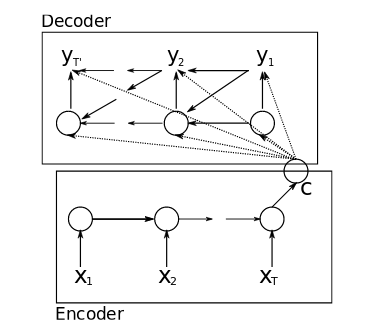
\includegraphics[width=0.5\textwidth]{RNN_encoder-decoder.png}
    \caption{neural network architecture}
    \label{fig:RNN_encoder-decoder}
\end{figure}
applications: machine translation, learning to excute, image captioning, conversational modeling

RNN Encoder-Decoder, consists of two recurrent neural networks (RNN) that act as an encoder and a decoder pair. The encoder maps a variable-length source sequence to a fixed-length vector, and the decoder maps the vector representation back to a variable-length target sequence. \cite{ChoLearningTranslation} also known as sequence embedding.

Why RNN encoder-decoder

The point of training an autoencoder is to make an RNN learn how to compress a relatively long sequence into a limited, dense vector.

\subsubsection{LSTM}
LSTM, introduced in \cite{Hochreiter1997LongMemory}, addresses the problem of vanishing gradients by introducing a memory cell which ensures constant error flow and gating units. The inner working of LSTM are listed follows:
\begin{equation}
	\begin{split}
		& \mathbf g^u = \sigma(\mathbf W^u * \mathbf h_{t-1} + \mathbf I^u * \x_t) \\
		& \mathbf g^f = \sigma(\mathbf W^f * \mathbf h_{t-1} + \mathbf I^f * \x_t) \\
		& \mathbf g^o = \sigma(\mathbf W^o * \mathbf h_{t-1} + \mathbf I^o * \x_t) \\
		& \mathbf g^c = \tanh(\mathbf W^c * \mathbf h_{t-1} + \mathbf I^c * \x_t) \\
		& \mathbf m_t = \mathbf g^f \odot \mathbf +  \mathbf g^u \odot \mathbf g^c \\
		& \mathbf h_t = \tanh(\mathbf g^o \odot \mathbf m_{t-1})
	\end{split}
\end{equation}


\subsection{lstm auto-encoder}
Autoencoders are data-specific. Autoencoders are lossy. Autoencoders are learned automatically from data examples, which is a useful property: it means that it is easy to train specialized instances of the algorithm that will perform well on a specific type of input. It doesn't require any new engineering, just appropriate training data. \cite{BuildingKeras}

An autoencoder contains: an encoding function, a decoding function, and a distance function between the amount of information loss between the compressed representation of your data and the decompressed representation (i.e. a "loss" function). The encoder and decoder will be chosen to be parametric functions (typically neural networks), and to be differentiable with respect to the distance function, so the parameters of the encoding/decoding functions can be optimize to minimize the reconstruction loss, using Stochastic Gradient Descent. It's simple! And you don't even need to understand any of these words to start using autoencoders in practice. \cite{BuildingKeras}

Today two interesting practical applications of autoencoders are data denoising (which we feature later in this post), and dimensionality reduction for data visualization. With appropriate dimensionality and sparsity constraints, autoencoders can learn data projections that are more interesting than PCA or other basic techniques. \cite{BuildingKeras}

\cite{MalhotraLongSeries} applied in time series. Long Short-Term Memory (LSTM) is able to solve many time series tasks unsolvable. by feedforward networks using fixed size time windows\cite{Gers2001ApplyingApproaches}.

LSTM attention\cite{BahdanauNEURALTRANSLATE};applied in time series \cite{CinarPosition-basedRNNs} \cite{QinAPrediction}

\begin{figure}[h]
    \centering
    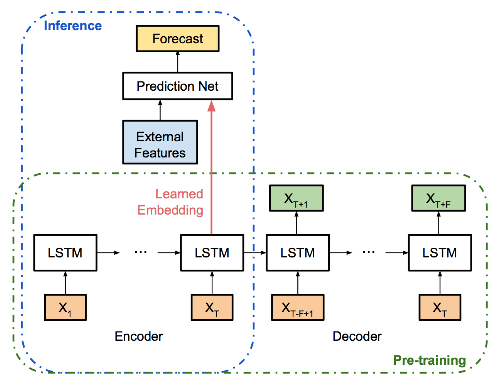
\includegraphics[width=0.5\textwidth]{neural_network_architecture.png}
    \caption{neural network architecture}
    \label{fig:neural_network_architecture}
\end{figure}
As you can see in the figure \ref{fig:neural_network_architecture}, the 
function grows near 0. Also, in the page \pageref{fig:neural_network_architecture} 
is the same example.
\section{implementation}
kafka, spark streaming 

tensorflow:\cite{TensorFlow}

online/offline training
\begin{figure}[h]
    \centering
    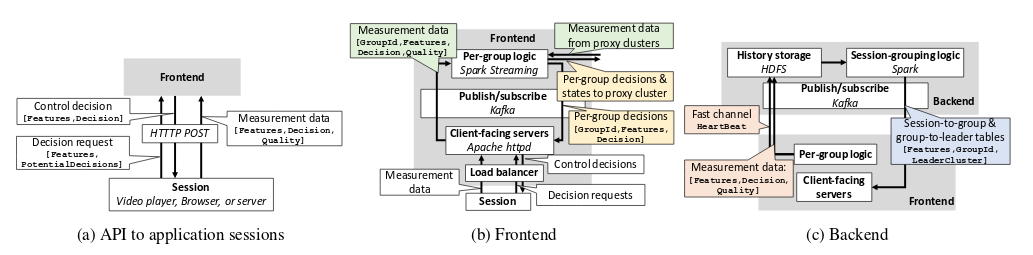
\includegraphics[width=1\textwidth]{implementation.png}
    \caption{implementation}
    \label{fig:implementation}
\end{figure}

\section{Evaluation}
\subsection{Experimental Settings}
data description

how samples are constructed

\subsection{Baseline}

\begin{enumerate}
  \item Persistent Model: a naive model that takes last ouput as the prediction
  \item Single-LSTM
  \item LSTM encoder-decoder with multiple-layers perceptions
  \item LSTM encoder-decoder with multiple-layers perceptions and attention
\end{enumerate}


\subsection{Performance}
\begin{table}[]
\centering
\caption{My caption}
\label{my-label}
\begin{tabular}{lllll}
location & Persistent & LSTM & LSTM encoder-decoder & Our model \\
Shanghai & 10.0       & 9.9  & 8.8                  & 7.7       \\
Shenzhen & 10.0       & 9.9  & 8.8                  & 7.7       \\
Zhejiang & 10.0       & 9.9  & 8.8                  & 7.7      
\end{tabular}
\end{table}



compare four different models in terms of training time and accuracy 
\subsection{Deployed at ChinaNetCenter}
\section{Discussion and Future Work}
a unified models for different cache groups.

further improve accuracy

uncertainty

qualified rate is an indirect measurement;collecting client data.

change detection
\section{Related Work}
edge-computing performance.\cite{SatyanarayananTheComputing}

data-driven networking. there are data-driven mechanisms

CDN: two types: long-term, short term;CDN selection \cite{Jiang2017Pytheas:Exploration-Exploitation}

deep-learning;RNN;RNN encoder-decoder;LSTM;LSTM time-series application;LSTM with attention

Geo-distributed data analytics:

deep learning and streaming data \cite{Najafabadi2015DeepAnalytics} incremental feature learning and ex traction, denoising autoencoders, and deep belief networks


Our work:
    \cite{Wang2017}

\section{Conclusion}
This paper shows that it is feasible to apply state-of-the-art Deep RL techniques to large-scale networked systems that provides esimation for its performance. Using the LSTM encoder-decoder with added machiene learning predictors offer a modeling selection for similar problems.
\section*{References}

\bibliographystyle{unsrt}
\bibliography{mendeley}

\end{document}